\documentclass[../../main.tex]{subfiles}

\begin{document}

\subsection{Verkettung von Abbildungen}
\label{sec:abbildungen_verkettung}

Abbildungen übersetzen Argumente, die aus ihrer Definitionsmenge kommen, in ihr jeweiliges Bild. Auf diese Weise erhält man bei einer Abbildung $f\colon U\rightarrow V$ Bilder aus der Menge $V$. Wie im folgenden Beispiel kommt es manchmal vor, dass nach Anwendung einer Abbildung direkt eine zweite Abbildung angewandt werden soll.

\begin{example}
    \parpic[r]{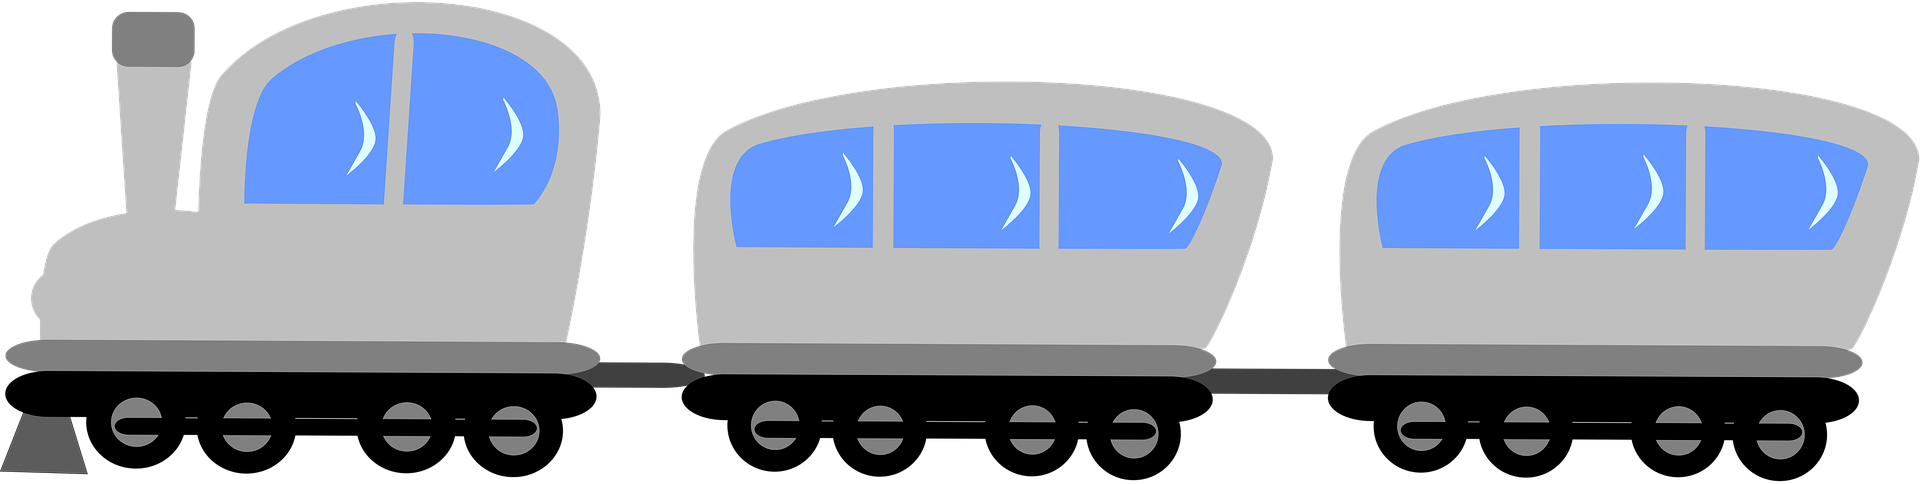
\includegraphics[width=.33\textwidth]{images/train.png}}
    Eine Gruppe von sechs Freunden möchte sich in Hamburg-Niendorf treffen. Zwei von ihnen wohnen außerhalb von Hamburg. Deswegen steigen sie zunächst in einen Zug, der sie zum Hamburger Hauptbahnhof fährt. Nach der Ankunft steigen die beiden um und fahren mit der U-Bahn weiter, bis sie ihre Freunde im Stadtteil Niendorf treffen.
    
    \picskip{0}
    Der Zug transportiert alle, die bis zur Endstation fahren, zum Hauptbahnhof (und beschreibt auf diese Weise eine Abbildung $\textsc{ZugNachHamburg}$, die alle Orte, an denen Gäste einsteigen, auf den Ort \emph{Hamburg Hbf.} abbildet). Die Straßenbahn nach Niendorf transport die beiden Freunde vom Hauptbahnhof nach Niendorf (also beschreibt sie eine Abbildung $\textsc{BahnNachNiendorf}$, die den Ort \emph{Hamburg Hbf.} auf \emph{Niendorf} abbildet).
    
    Wenn einer der Freunde in Itzehoe (einer Stadt nördlich von Hamburg) in den Zug nach Hamburg steigt und dann in die U-Bahn, dann gelangt er nach Niendorf. Auf seinen Ausgangsort \emph{Itzehoe} hat er erst die Abbildung $\textsc{ZugNachHamburg}$ angewandt ($\textsc{ZugNachHamburg}(\emph{Itzehoe})=\emph{Hamburg Hbf.}$) und anschließend durch das Einsteigen in die Straßenbahn die Abbildung $\textsc{BahnNachNiendorf}$ genutzt, um nach Niendorf zu kommen ($\textsc{BahnNachNiendorf}(\emph{Hamburg Hbf.})=\emph{Niendorf}$).
\end{example}

Bei der Hintereinanderausführung (oder \textbf{Komposition}) von Abbildungen geht es darum, ein Argument mithilfe einer Abbildung auf sein Bild abzubilden (so, wie du das bereits aus den letzten Abschnitten kennst) und anschließend das erhaltene Bild direkt in eine zweite Abbildung einzusetzen und erneut abzubilden. Auf diese Weise wird jedes Element aus der Definitionsmenge der ersten Abbildung -- mit einem Zwischenschritt -- auf ein Element aus der Bildmenge der zweiten Abbildung abgebildet.

\begin{example}
    Der Freund, der aus Itzehoe nach Niendorf gefahren ist, hat zwei Abbildungen hintereinander ausgeführt. Er ist erst mit dem Zug nach Hamburg gefahren und anschließend mit der U-Bahn zu seinem Ziel in Niendorf. Mathematisch aufgeschrieben gilt \[\textsc{BahnNachNiendorf}(\underbrace{\textsc{ZugNachHamburg}(\emph{Itzehoe})}_{\emph{Hamburg Hbf.}})=\emph{Niendorf}.\]
\end{example}

Mathematisch funktioniert die Hintereinanderausführung so, dass man ein Argument $x$ zunächst benutzt, um $f(x)$ zu berechnen, d.h. um es mithilfe von $f$ abzubilden. Anschließend setzt man dieses Ergebnis in eine Abbildung $g$ ein. Man berechnet also $g(f(x))$. $f(x)$ wird an dieser Stelle als Argument für $g$ verwendet.

\begin{figure}[h!]
    \centering
    \begin{tikzpicture}[scale=.75]
    \draw[grayset] (-1.5,0) ellipse (0.7cm and 2cm);
    \draw[grayset] (1.5,0) ellipse (0.7cm and 2cm);
    \draw[grayset] (4.5,0) ellipse (0.7cm and 2cm);

    \node[red] (x1) at (-1.5,0.7) {$\bullet$};
    \node (x2) at (-1.5,-0.2) {$\bullet$};
    \node (x3) at (-1.5,-1.1) {$\bullet$};
    \node (y1) at (1.5,0.7) {$\bullet$};
    \node (y2) at (1.5,-0.2) {$\bullet$};
    \node[violet] (y3) at (1.5,-1.2) {$\bullet$};
    \node (z1) at (4.5,1.2) {$\bullet$};
    \node (z2) at (4.5,0.4) {$\bullet$};
    \node (z3) at (4.5,-0.4) {$\bullet$};
    \node[blue] (z4) at (4.5,-1.2) {$\bullet$};

    \draw[->] (x1) -- (y3);
    \draw[->] (x2) to[bend right] (y1);
    \draw[->] (x3) to[bend right] (y2);
    
    \draw[->] (y1) -- (z3);
    \draw[->] (y2) -- (z1);
    \draw[->] (y3) -- (z4);
    
    \node at (0,1) {$f$};
    \node at (3,1) {$g$};
\end{tikzpicture}
    \caption{Ein Element der links dargestellten Menge kann mit der eingezeichneten Abbildung $f$ in ein Element der mittleren Menge übersetzt werden (z.B. kann das rote auf das violette Element abgebildet werden). Das violette Element kann mithilfe der zweiten eingezeichneten Abbildung $g$ auf ein Element der rechten Menge abgebildet werden, und zwar auf das blaue. Das heißt, dass das rote Element insgesamt mit einem Zwischenschritt auf das blaue abgebildet wird, wenn man erst die linke und dann die rechte Abbildung anwendet. Dafür hat man zunächst $f(x)$ berechnet und das Ergebnis anschließend in die Abbildung $g$ eingesetzt, also $g(f(x))$ berechnet.}
\end{figure}

Zwei Abbildungen hintereinander auszuführen klappt nur dann, wenn die zweite Abbildung etwas mit den Ergebnissen der ersten anfangen kann (also für sie definiert ist). Im folgenden Bild siehst du, wie die zweite Abbildung genau dort ansetzt, wo die erste aufhört. Neben das Abbildungsdiagramm der ersten Abbildung wird ein zweites Abbildungsdiagramm gezeichnet. Dabei teilen sich beide Abbildungen eine Menge: Die zweite Abbildung nutzt die Bildmenge der ersten als ihre Definitionsmenge.

So ist es möglich, dass -- wie an einem Fließband in einer Fabrik -- erst die Abbildung $f$ ein Argument erhält und es in ein Bild übersetzt, mit dem $g$ weiterarbeiten kann. Anschließend erhält $g$ dieses Bild und verarbeitet es seinerseits weiter.

\begin{example}
    \parpic[r]{
        \begin{tikzpicture}
            \draw[black!25,fill=black!10] (-1.5,0) circle[radius=6mm];
            \draw[black!25,fill=black!10] (0,0) circle[radius=6mm];
            \draw[black!25,fill=black!10] (1.5,0) circle[radius=6mm];
            %node content
            \node[yellow!70!black] at (-1.5,0) {\euro};
            \node[yellow!70!black] at (0,0) {\$};
            \node[yellow!70!black] at (1.5,0) {
\includegraphics[height=10mm]{images/statue_of_liberty.png}};
            %connection lines
            \draw[very thick,black!40,->] (-1.5,0.6) to[bend left] (0,0.6);
            \draw[very thick,black!40,->] (0,-0.6) to[bend right] (1.5,-0.6);
        \end{tikzpicture}
    }
    Bei einer Reise in die USA, in denen man mit der Währung Dollar bezahlt, kann man als Europäer natürlich nicht mit Euro bezahlen. Wer dorthin reist, wechselt deshalb vorher etwas Geld, das er für die Reise einplant, in Dollar.
    \picskip{2}
    
    Mit diesem Geld ist es anschließend unter anderem möglich, vor Ort Essen in Restaurants zu kaufen sowie den Eintritt zu Sehenswürdigkeiten und anderen Touristenattraktionen zu bezahlen. Wir gehen nun davon aus, dass von dem Geld Tickets für den Besuch der Freiheitsstatue gekauft werden sollen (Preis: 40\,\$).
    
    Für einen USA-Urlaub wechselt man also erst seine Euro in Dollar und anschließend die Dollar in Eintrittskarten, Verpflegung und ähnliches. Wir wissen bereits, dass sich das Wechseln von Euro in Dollar als eine Abbildung beschreiben lässt. Angenommen, der Wechselkurs liegt bei $1.2\:\$$, die man pro Euro bekommt. Dann ordnet die Abbildung $\textsc{Dollar}\colon\Real\rightarrow\Real$ mit der Abbildungsvorschrift $\textsc{Dollar}(x)=1.2x$ dem investierten Betrag in Euro zu, wie viele Dollar man dafür erhält. Es gilt beispielsweise $\textsc{Dollar}(5)=6$, weil man 6 Dollar für 5 Euro erhalten würde.
    
    Die Abbildung $\textsc{TicketsFürDollar}\colon\Real\rightarrow\Integer$ könnte nun beschreiben, wie viele Tickets man für einen bestimmten Betrag (in Dollar) kaufen kann.
    
    Möchte man nun wissen, wie viele Tickets für die Freiheitsstatue für 100\,€ erhältlich sind, muss man diesen Betrag zunächst in Dollar umrechnen (mithilfe der Abbildung $\textsc{Dollar}$). Es gilt $\textsc{Dollar}(100)=120$. Anschließend verrät die Abbildung $\textsc{TicketsFürDollar}$, dass man $3$ Tickets kaufen kann, weil man die eben erhaltene $120$ einsetzt und $\textsc{TicketsFürDollar}(120)=3$ gilt.
    
    Wir haben erst $\textsc{Dollar}(100)$ und dann $\textsc{TicketsFürDollar}(120)$ berechnet. Die $120$ ist genau das Ergebnis von $\textsc{Dollar}(100)$. Also ist \[\textsc{TicketsFürDollar}(120)=\textsc{TicketsFürDollar}(\underbrace{\textsc{Dollar}(100)}_{=120}).\]
    
    Um zu berechnen, wie viele Tickets wir für $x$ Euro bekommen, berechnen wir also $\textsc{TicketsFürDollar}(\textsc{Dollar}(x))$.
\end{example}

Zwei Abbildungen $f$ und $g$ nacheinander anzuwenden, kann sich manchmal als sinnvoll erweisen, wenn man mit einfachen Zwischenschritten zu einem bestimmten Ergebnis kommt, statt eine kompliziertere Abbildung in einem Schritt zu berechnen.

\begin{example}
    Wenn man im Kopf für eine bestimmte Zahl $x$ den Wert $3x+2$ ausrechnen möchte, dann kann man das nicht sinnvoll in einem Schritt tun. Stattdessen wirst du dir erst überlegen, was $3x$ ist. Anschließend wirst du $2$ zum Ergebnis addieren. In einem ersten Schritt berechnest du also die Abbildung $f(x)=3x$, die die Addition von $2$ zunächst ignoriert.
    
    Nachdem du weißt, welchen Wert $3x$ hat, addierst du darauf $2$. Mit der Abbildung $g(x)=x+2$ tust du genau das. Führst du beide Abbildungen hintereinander aus, berechnest du \[g(f(x))=g(3x)=3x+2,\] also genau das, was du berechnen wolltest -- nur mit einem Zwischenschritt.
    
    Für $x=5$ gilt zum Beispiel $f(5)=3\cdot 5=15$ und $g(f(5))=g(15)=15+2=17$. Natürlich ist auch \[\overbrace{\underbrace{3\cdot 5}_{f(5)}+2}^{g(f(5))}=17.\]
\end{example}

Gerade im letzten Beispiel hat man gesehen, dass auch das Hintereinanderausführen von zwei Abbildungen selbst wieder eine Abbildung ist. Jedes Argument für $f$ wird eindeutig erst auf ein Argument für $g$ und dann auf das Bild, das $g$ produziert, abgebildet. Die Abbildung $g(f(x))$ kann daher selbst als eine Abbildung definiert werden. Sie wird die \textbf{Verkettung} oder die \textbf{Komposition} von $f$ und $g$ genannt.

\begin{definition}[Verkettung von Abbildungen]
    Es seien $U,V,W$ Mengen und $f\colon U\rightarrow V$ sowie $g\colon V\rightarrow W$ Abbildungen.
    
    Die Abbildung $g\circ f\colon U\rightarrow W$ mit \[x\mapsto (g\circ f)(x)\coloneqq g(f(x))\] heißt die \textbf{Komposition} oder \textbf{Verkettung} von $f$ und $g$.
\end{definition}

Die Abbildung $g\circ f$ bildet ihre Argumente auf das Bild ab, das man erhält, wenn man erst $f$ und dann $g$ anwendet. Hierbei sollte man sich nicht davon verwirren lassen, dass das $g$ links steht -- das $f$ wird trotzdem zuerst angewandt, denn es befindet sich bei der Schreibweise $g(f(x))$ innen. Die Schreibweise $g\circ f$ aus dieser Definition kann man als \enquote{$g$ Kringel $f$} lesen.

Die Reihenfolge, in der man $f$ und $g$ anwendet, ist für Verkettungen sehr wichtig. Einerseits kann es sein, dass man, wenn man erst $g$ anwendet, überhaupt kein Bild erhält, das in der Definitionsmenge von $f$ liegt. Es ist aber auch selbst dann, wenn die Definitions- und Bildmengen dennoch zu einander passen, nicht egal, in welcher Reihenfolge man die Abbildungen anwendet (wie im nächsten Beispiel zu sehen ist).

\begin{example}
    Im letzten Beispiel haben wir gesehen, dass $g(f(x))=3x+2$ ist. Die Verkettung dieser beiden Abbildungen $g\circ f$ ist die Abbildung $(g\circ f)(x)=3x+2$.
    
    Es gilt hingegen aber $(f\circ g)(x)=f(g(x))=f(x+2)=3(x+2)=3x+6$. Die Reihenfolge, in der man $f$ und $g$ anwendet, ist also sehr wichtig und verändert die Abbildung, die man bei der Verkettung erhält.
\end{example}

\begin{nutshell}{Verkettung von Abbildungen}
    \parpic[r]{\begin{tikzpicture}[scale=.6]
    \draw[grayset] (-1.5,0) ellipse (0.7cm and 2cm);
    \draw[grayset] (1.5,0) ellipse (0.7cm and 2cm);
    \draw[grayset] (4.5,0) ellipse (0.7cm and 2cm);

    \node (x1) at (-1.5,0.7) {$\bullet$};
    \node (x2) at (-1.5,-0.2) {$\bullet$};
    \node (x3) at (-1.5,-1.1) {$\bullet$};
    \node (y1) at (1.5,0.7) {$\bullet$};
    \node (y2) at (1.5,-0.2) {$\bullet$};
    \node (y3) at (1.5,-1.2) {$\bullet$};
    \node (z1) at (4.5,1.2) {$\bullet$};
    \node (z2) at (4.5,0.4) {$\bullet$};
    \node (z3) at (4.5,-0.4) {$\bullet$};
    \node (z4) at (4.5,-1.2) {$\bullet$};

    \draw[->] (x1) -- (y3);
    \draw[->] (x2) to[bend right] (y1);
    \draw[->] (x3) to[bend right] (y2);
    
    \draw[->] (y1) -- (z3);
    \draw[->] (y2) -- (z1);
    \draw[->] (y3) -- (z4);
    
    \node at (0,1) {$f$};
    \node at (3,1) {$g$};
\end{tikzpicture}}
    Zwei Abbildungen $f$ und $g$, bei denen $f$ seine Argumente in die Definitionsmenge von $g$ abbildet, können hintereinander angewandt werden. Dafür bildet man ein Element $x$ der Definitionsmenge von $f$ erst mit $f$ und das Ergebnis $f(x)$ dann mit $g$ ab. Man berechnet also $g(f(x))$.
      
    \picskip{0} 
    Die Abbildung, die jedes Element aus der Definitionsmenge von $f$ auf das Element der Bildmenge von $g$ abbildet, das man erhält, wenn man erst $f$ und dann $g$ anwendet, heißt \textbf{Verkettung} von $f$ und $g$. Sie wird geschrieben als $g\circ f$. Es gilt also $(g\circ f)(x)=g(f(x))$.
\end{nutshell}

\subsection{Die Identische Abbildung}
\label{sec:abbildungen_identitaet}

In der Regel verändern Abbildungen ihre Argumente, indem sie diese auf ihre Bilder abbilden. Eine solche Zuordnung von Elementen der Definitionsmenge zu Elementen der Bildmenge ist schließlich der Zweck von Abbildungen. 

Es ist jedoch nicht verboten, mit Abbildungen, die gar nichts tun, zu arbeiten. Damit sind Abbildungen gemeint, die ihr Argument nicht verändern. Das heißt, jedes Argument, das man in die Abbildung einsetzt, wird auf sich selbst abgebildet.

\begin{example}
    \parpic[r]{%\begin{center}
    \begin{tikzpicture}[scale=.6]
        \fill[black!10] (-1.5,0) ellipse (2.4cm and 2cm);
        \fill[black!10] (4,0) ellipse (2.4cm and 2cm);
        %
        \draw (-1.5,0) ellipse (2.4cm and 2cm);
        \draw (4,0) ellipse (2.4cm and 2cm);
        %
        \node[blue] (x1) at (-1,0.7) {$\bullet$}; 
        \node[blue,left=1mm of x1] {blau};
        \node[red] (x2) at (-1,-0.2) {$\bullet$}; 
        \node[red,left=1mm of x2] {rot};
        \node[yellow!70!black] (x3) at (-1,-1.1) {$\bullet$}; 
        \node[yellow!70!black,left=1mm of x3] {gelb};
        %
        \node[blue] (y1) at (3.5,0.7) {$\bullet$}; 
        \node[blue,right=1mm of y1] {blau};
        \node[red] (y2) at (3.5,-0.2) {$\bullet$}; 
        \node[red,right=1mm of y2] {rot};
        \node[yellow!70!black] (y3) at (3.5,-1.1) {$\bullet$}; 
        \node[yellow!70!black,right=1mm of y3] {gelb};
        %
        \draw[->] (x1) to[bend left] (y1);
        \draw[->] (x2) -- (y2);
        \draw[->] (x3) to[bend right] (y3);
    \end{tikzpicture}
%\end{center}}
    Wir hatten bereits die Abbildung $\textsc{MitGelbMischen}$ gesehen, die Grundfarben erhält und mit gelb mischt. Dadurch verändern sich die Farben blau zu grün und rot zu orange. Deutlich langweiliger ist es, eine Grundfarbe mit sich selbst zu mischen, also blau mit blau, rot mit rot und gelb mit gelb. Natürlich ändert eine Farbe sich nicht, wenn man sie mit sich selbst mischt.
    
    \picskip{0}
    Es lässt sich eine Abbildung $\textsc{MitSichSelbstMischen}$ definieren, bei der jede Grundfarbe auf die Farbe abgebildet wird, die entsteht, wenn man die Grundfarbe mit sich selbst mischt. Weil das wie bereits beschrieben die Farbe nicht ändert, erhält man dadurch eine Abbildung
    \[\textsc{MitSichSelbstMischen}\colon\textsc{Grundfarben}\rightarrow\textsc{Grundfarben}\]
    mit
    \[\textsc{MitSichSelbstMischen}(x)=x.\]
\end{example}

Eine Abbildung mit dieser Eigenschaft wird \textbf{identische Abbildung} genannt. Der Name kommt daher, dass Urbild und Bild immer identisch sind. Eine identische Abbildung gibt es für jede Definitionsmenge (das ist dann immer die Abbildung, die alle Elemente dieser Menge auf sich selbst abbildet).

\begin{definition}[Identische Abbildung]
    Es sei $M$ eine Menge. Dann heißt die Abbildung, die jedes Element von $M$ auf sich selbst abbildet, die \textbf{identische Abbildung} oder \textbf{Identität} auf $M$, geschrieben $\ident[M]$. Es gilt also \[\ident[M](x)=x\text{~für alle~}x\in M.\]
\end{definition}

Die identische Abbildung auf einer Menge $M$ notiert man also mit $\ident[M]$. Meistens lässt man die Menge im Index weg, schreibt also einfach nur $id$, wenn klar ist, um welche Menge es geht. Wir werden die Menge hier allerdings zur Klarheit weiterhin mit aufschreiben.

\subsection{Die Umkehrabbildung}
\label{sec:abbildungen_umkehrabbildung}

Im letzten Abschnitt hast du gesehen, dass identische Abbildungen solche Abbildungen sind, die ihre Argumente nicht verändern, sondern einfach auf sich selbst abbilden. Eine solche Abbildung anzuwenden, hat keinen Effekt, denn sie verändert nichts.

Dieser Abschnitt thematisiert die Frage, ob es möglich ist, wenn man bereits eine Abbildung $f$ angewandt hat, anschließend eine andere Abbildung $g$ anzuwenden, die den Effekt von $f$ umkehrt. Das heißt, dass wenn man zuerst $f$ und dann $g$ anwendet, insgesamt nichts passiert. Ist $f$ eine Abbildung von $U$ nach $V$ ($U,V$ sind Mengen), dann ist also eine Abbildung $g\colon V\rightarrow U$ gesucht, sodass bei der Hintereinanderausführung von $f$ und $g$ die identische Abbildung herauskommt.

\begin{figure}[ht]
    \centering
    \begin{tikzpicture}[scale=.75]
    \draw[grayset] (-1.5,0) ellipse (0.7cm and 2cm);
    \draw[grayset] (1.5,0) ellipse (0.7cm and 2cm);

    \node (x1) at (-1.5,0.7) {$\bullet$};
    \node (x2) at (-1.5,-0.2) {$\bullet$};
    \node (x3) at (-1.5,-1.1) {$\bullet$};
    \node (y1) at (1.5,0.7) {$\bullet$};
    \node (y2) at (1.5,-0.2) {$\bullet$};
    \node (y3) at (1.5,-1.2) {$\bullet$};

    \draw[blue,->] (x1) -- (y3);
    \draw[blue,->] (x2) to[bend right] (y1);
    \draw[blue,->] (x3) to[bend right] (y2);
    
    \draw[dashed,->] (y3) to[bend right] (x1);
    \draw[dashed,->] (y1) to[bend right] (x2);
    \draw[dashed,->] (y2) to[bend right] (x3);
\end{tikzpicture}
    \caption{In diesem Abbildungsdiagramm ist die Abbildung $f$ mit blauen Pfeilen dargestellt. Die gestrichelte Abbildung dreht alle Pfeile von $f$ um. Dadurch läuft man immer im Kreis, wenn man erst einem blauen und dann einem gestrichelten Pfeil folgt. Führt man die beiden Abbildungen hintereinander aus, bekommt man deshalb die identische Abbildung auf der linken Menge.}
\end{figure}

\begin{example}
    Die Abbildung $f\colon\Real\rightarrow\Real$ mit der Abbildungsvorschrift $f(x)=x+1$ addiert zu jeder Zahl 1. Wenn man vom Ergebnis wieder $1$ subtrahiert, kommt man bei der Zahl an, bei der man angefangen hat. Für die Abbildung $g\colon\Real\rightarrow\Real$ mit $g(x)=x-1$ gilt also $(g\circ f)(x)=x$. Das lässt sich nachrechnen:
    \[g(f(x))=g(x+1)=(x+1)-1=x.\]
    Die Abbildung $g$ kehrt die Abbildung $f$ daher um und es gilt $g\circ f=\ident[\Real]$.
\end{example}

Eine Abbildung $g$, die eine Abbildung $f\colon U\rightarrow V$ rückgängig macht bzw. umkehrt, wird Umkehrabbildung von $f$ genannt. Wie eben erklärt, drückt sich das dadurch aus, dass bei der Hintereinanderausführung von $f$ und $g$ die identische Abbildung herauskommt, also $g\circ f=\ident[U]$. Dass $g$ eine Abbildung von $V$ nach $U$ sein muss, ist erzwungen: Die Definitionsmenge muss $V$ sein, damit die Abbildungen überhaupt hintereinander ausgeführt werden dürfen. Die Bildmenge von $g$ muss $U$ sein, weil man bei Elementen aus $U$ begonnen hat und entsprechend auch wieder zu Elementen aus $U$ zurück möchte.

\begin{definition}[Umkehrabbildung]
    Es seien $U,V$ Mengen und $f\colon U\rightarrow V$ eine Abbildung. Eine Abbildung $g\colon V\rightarrow U$ mit $g\circ f=\ident[U]$ und $f\circ g=\ident[V]$ heißt \textbf{Umkehrabbildung} von $f$. In diesem Fall schreibt man $f^{-1}$ statt $g$.
\end{definition}

Die Umkehrabbildung einer Abbildung $f$ notiert man mit $f^{-1}$. Im nächsten Beispiel wird noch einmal erläutert, warum $g$ im letzten Beispiel eine Umkehrabbildung von $f$ war. Anschließend werden zwei weitere Beispiele präsentiert.

\begin{example}
    Im letzten Beispiel haben wir gesehen, dass für $f\colon\Real\rightarrow\Real$ mit $f(x)=x+1$ die Umkehrabbildung durch $f^{-1}(x)=x-1$ bestimmt ist. Es gilt nämlich $g\circ f=\ident[\Real]$. Außerdem gilt $f\circ g=\ident[\Real]$, weil $f(g(x))=f(x-1)=(x-1)+1$ gilt.
\end{example}

\begin{example}
    Wenn ein mit Butter beschmiertes Toast von einem normalen Tisch nach unten fällt, landet es leider oft mit der beschmierten Seite unten. Während des Falls kann das Toast sich prinzipiell mehrmals drehen. Nach jedem Drehen zeigt entweder die Seite mit Butter oder die Seite ohne Butter nach oben.
    
    Die Abbildung $\textsc{Umdrehen}\colon\textsc{Toastseiten}\rightarrow\textsc{Toastseiten}$ gibt nun an, welche Seite des Toasts nach dem Umdrehen oben ist, abhängig davon, welche vorher oben war (wobei $\textsc{Toastseiten}$ die Menge der Seiten ist, die sich prinzipiell oben befinden können, d.h. $\textsc{Toastseiten}=\{\text{Butter},\text{keine Butter}\}$). Es gilt (weil sich nach einmaligem Umdrehen jeweils die andere Seite oben befindet)
    \[\textsc{Umdrehen}(\text{Butter})=\text{keine Butter}\] und \[\textsc{Umdrehen}(\text{keine Butter})=\text{Butter}.\]
    Wenn sich das Toast zweimal umdreht, ist wieder die Seite oben, die vorher oben war, d.h. \[\textsc{Umdrehen}(\textsc{Umdrehen}(\text{keine Butter}))=\textsc{Umdrehen}(\text{Butter})=\text{keine Butter}\]
    und auf die gleiche Weise liegt auch die Seite mit Butter oben, wenn vorher die Seite mit Butter oben war und sich das Toast zweimal umdreht. Damit ist das zweimalige Umdrehen des Toasts die identische Abbildung auf der Menge \textsc{Toastseiten}. Weil $\textsc{Umdrehen}\circ \text{Umdrehen}=\ident[\textsc{Toastseiten}]$ gilt, ist \textsc{Umdrehen} die Umkehrabbildung von sich selbst.
\end{example}

\begin{example}
    Die Abbildung $f\colon\Real\rightarrow\Real$ mit $f(x)=4x$ hat die Umkehrabbildung $f^{-1}\colon\Real\rightarrow\Real$ mit $f^{-1}(x)=\frac{1}{4}x$: Um eine Multiplikation mit $4$ rückgängig zu machen, muss man durch $4$ teilen (oder mit $\frac{1}{4}$ multiplizieren).
    
    Zur Überprüfung lässt sich schnell nachrechnen, dass \[(f^{-1}\circ f)(x)=f^{-1}(f(x))=f^{-1}(4x)=\frac{1}{4}\cdot 4x=x.\] 
    Damit ist $f^{-1}\circ f=\ident[\Real]$. Natürlich kann ebenso gezeigt werden, dass $f\circ f^{-1}=\ident[\Real]$ ist.
\end{example}

\begin{nutshell}{Identität und Umkehrabbildung}
    \sloppy
    Eine \textbf{identische Abbildung} auf einer Menge $M$ (geschrieben $id_M$) ist eine Abbildung, die als Definitions- und Bildmenge $M$ hat und alle Argumente unverändert lässt, d.h. $f(x)=x$ für alle $x\in M$. Damit handelt es sich um eine Abbildung, die nichts tut.
    
    Wenn es möglich ist, zu einer Abbildung $f\colon U\rightarrow V$ eine Abbildung $g\colon V\rightarrow U$ zu finden, sodass diese sich gegenseitig rückgängig machen (also $g\circ f=\ident[U]$ und $f\circ g=\ident[V]$), dann nennt man $g$ die \textbf{Umkehrabbildung} von $f$ und schreibt für $g$ auch $f^{-1}$.
\end{nutshell}

\fussy
\begin{advanced}{Injektionen, Surjektionen und Bijektionen}
    Wenn man die Abbildungsvorschrift einer Abbildung weiter analysieren möchte, ist eine wichtige Eigenschaft, wie viele Urbilder die Elemente der Bildmenge jeweils haben. Man stellt sich in diesem Zusammenhang die Frage, ob
    \begin{itemize}[noitemsep]
        \item jedes Element der Bildmenge mindestens ein Urbild hat oder
        \item jedes Element der Bildmenge maximal ein Urbild hat oder
        \item jedes Element der Bildmenge genau ein Urbild hat.
    \end{itemize}
    
    Eine Abbildung heißt im ersten Fall \textbf{surjektiv}, im zweiten Fall \textbf{injektiv} und im dritten Fall (wenn die Abbildung also sowohl injektiv als auch surjektiv ist) heißt sie \textbf{bijektiv}.
    
    \begin{definition}
        Eine Abbildung $f\colon U\rightarrow V$ heißt \textbf{surjektiv}, falls für jedes $v\in V$ ein $u\in U$ mit $f(u)=v$ existiert, d.h. wenn jedes Element der Bildmenge mindestens ein Urbild hat.
        
        Sie heißt \textbf{injektiv}, falls aus $f(u)=f(u')$ für beliebige $u,u'\in U$ stets folgt, dass $u=u'$ gilt. 
        
        Eine Abbildung heißt bijektiv, falls sie \textbf{surjektiv} und \textbf{injektiv} ist.
    \end{definition}
    
    Es ist auch möglich, dass eine Abbildung keine dieser Eigenschaften hat.
    Eine Erläuterung dieser Definition sowie Beispiele findest du am Ende dieses Kapitels auf Seite \pageref{advanced:bijektion}.
\end{advanced}

\end{document}